\section{Evaluation}\label{sec:eval}
Every number in this section comes from one run of \texttt{DEMO-ALL} and \texttt{BENCH} (Section~\ref{sec:setup}), scored against the answer key of 712 known weaknesses, and the tables and figures reproduce the comparison page that \texttt{BENCH} writes (\texttt{results/opensource/comparison.html}). The section answers five questions in turn. \textit{Speed} (Section~\ref{sec:eval-speed}) asks how long each tool takes to review one system, measured as the wall-clock time of one run on each system; for ATG we time both the scan process (Phases 1--4) and the whole scan. \textit{Computing resources} (Section~\ref{sec:eval-res}) asks how much CPU time, memory, disk and network each tool uses, from the operating system's counters for each tool's processes and Docker's counters for ATG's four containers. \textit{Accuracy} (Section~\ref{sec:eval-acc}) asks how many of the 712 known weaknesses each tool finds and how complete ATG's API inventory is; every tool's findings are translated into the 22 kinds of weakness and matched with the answer key by place. \textit{Systems covered} (Section~\ref{sec:eval-sys}) asks on how many of the ten systems each tool can run at all, and \textit{language limits} (Section~\ref{sec:eval-lang}) which services and programming languages each tool can review. In short, ATG's analysis takes 0.44~s per system (7.7~s for the whole scan) against 0.04--4.1~s for the file scanners, and one ATG scan uses 0.82~s of CPU and 144~MB at most, against 4.1~s and 761~MB for Checkov. ATG finds 462 of the 712 known weaknesses (65\%) with 75\% of its reports correct, while the best other tool, Polaris, finds 349 (49\%), and ATG lists 189 of the 201 operations. ATG runs on all ten systems and reviews all 65 services in eight languages, while each Kubernetes scanner runs on seven systems, Spectral on three and each code scanner on three or four, and the three code scanners together read 26 services (40\%).

\FloatBarrier
\subsection{Speed}\label{sec:eval-speed}
This part asks how long each tool takes to review one system. Table~\ref{tab:speed} and Fig.~\ref{fig:speed} give the median over the systems each tool can read, with the fastest and slowest system.

For ATG we report two times. The analysis itself (Phases 1--4, timed inside the ATG container) takes 0.44~s per system (0.23--0.88~s): Phase~1, which reads the four sources and probes for API documents, 0.20--0.69~s, Phase~2 2--8~ms, Phase~3 20--138~ms and Phase~4 3--43~ms. The whole scan takes 7.7~s (7.0--8.3~s); most of the difference is a fixed wait for the sidecar and the Collector to go quiet before ATG reads their buffers. Neither time includes starting the system or running its users, which \texttt{DEMO-ALL} does before the scan.

The other tools' time is one run of the tool on the system's files. They take 0.04~s (kube-linter) to 4.1~s (gosec) per system, and their time grows with what they read: gosec loads every Go package and took 34.1~s on Online Boutique, and Checkov took 12.7~s on Lakeside Mutual. The first run of each tool is slower because it loads its rules; the median is not affected by that one run. ATG's analysis is faster than six of the eight tools and slower than Polaris and kube-linter. With the wait, the whole scan is slower than every tool's median, and it took at most 8.3~s on any system.

\begin{table}[!htbp]
\caption{Time to review one system, slowest first. Systems: systems the tool can read}
\label{tab:speed}
\centering
\footnotesize
\setlength{\tabcolsep}{3pt}
\begin{tabular}{@{}>{\raggedright\arraybackslash}p{3.3cm}rrrr@{}}
\toprule
Tool & Systems & Median & Fastest & Slowest \\
\midrule
%%speed%%
\bottomrule
\end{tabular}
\end{table}

\begin{figure}[!htbp]
\centering
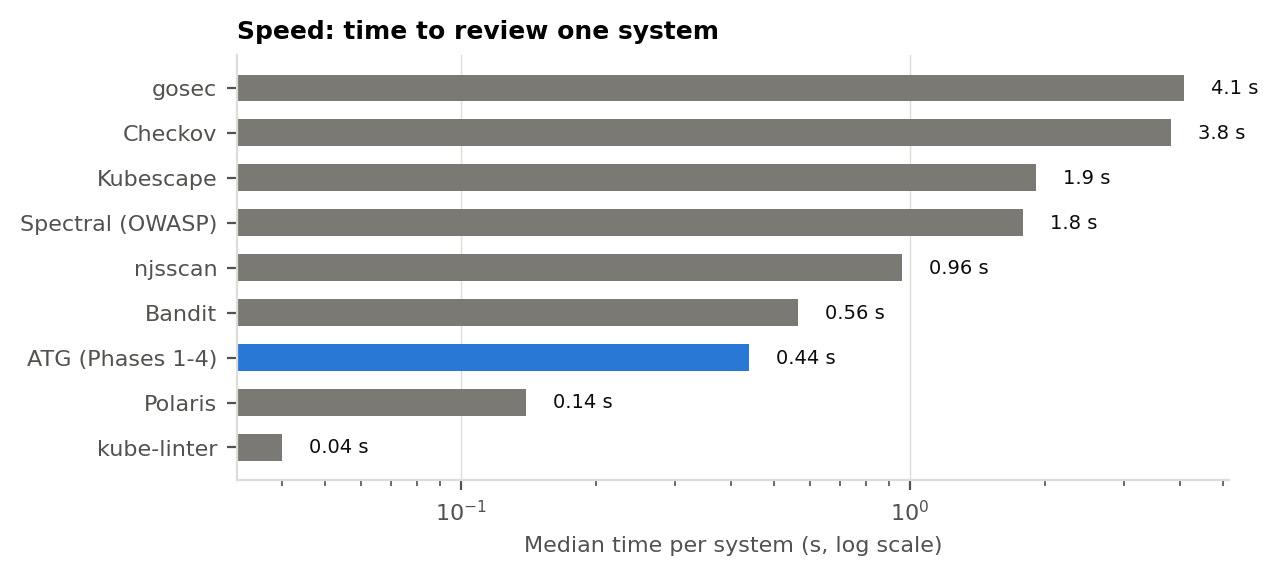
\includegraphics[width=\columnwidth]{figs/fig_speed.png}
\caption{Median time to review one system (log scale).}
\label{fig:speed}
\end{figure}

\FloatBarrier
\subsection{Computing resources}\label{sec:eval-res}
This part asks how much of the computer each tool uses to review one system (Table~\ref{tab:cost}, Figs.~\ref{fig:cpu} and~\ref{fig:mem}). The measures are defined in Section~\ref{sec:setup}.

During a scan, the ATG and PostgreSQL containers use 0.82~s of CPU time (0.71~s user, 0.11~s system) and hold 144~MB at most and 128~MB on average; the scan process reads 3.9~MB and writes 2.8~MB. Over the 7.7~s of the scan this keeps about a tenth of one core busy (0.11), because most of the scan is the wait described above. The file scanners keep about one core busy while they run (0.84--1.25). By median, kube-linter, Polaris and Bandit stay under 40~MB and half a second of CPU. Checkov uses the most memory, 761~MB per system, and gosec the most CPU time, 5.1~s per system. By median, ATG's scan uses less CPU time than four of the eight tools and more memory than all of them except Checkov.

\begin{table*}[!t]
\caption{Computing resources to review one system: median over the systems each tool can read. Sorted by the number of systems the tool can read, most first; tools that read the same number by CPU time}
\label{tab:cost}
\centering
\scriptsize
\setlength{\tabcolsep}{3.5pt}
\begin{tabular}{@{}>{\raggedright\arraybackslash}p{3.3cm}rrrrrrrrr@{}}
\toprule
Tool & Systems & CPU time & User / system & Cores used & Peak memory & Average memory & Data read & Data written & Processes \\
\midrule
%%cost%%
\bottomrule
\end{tabular}
\end{table*}

\textit{The largest use on one system.} The most CPU time and the highest peak memory any tool needed for one system were: gosec 48.1~s and 282~MB, both on Online Boutique, where it read 363~MB; Checkov 13.2~s on Lakeside Mutual and 954~MB on Online Boutique; Spectral 4.4~s on Lakeside Mutual and 132~MB; Kubescape 2.0~s and 124~MB, both on Hotel Reservation; ATG's scan 1.2~s on Online Boutique and 159~MB; njsscan 1.1~s and 92~MB, both on Robot Shop; Bandit 0.84~s and 32~MB, both on Bank of Anthos; Polaris 0.25~s and 38~MB; and kube-linter 0.05~s and 36~MB.

\begin{figure}[!htbp]
\centering
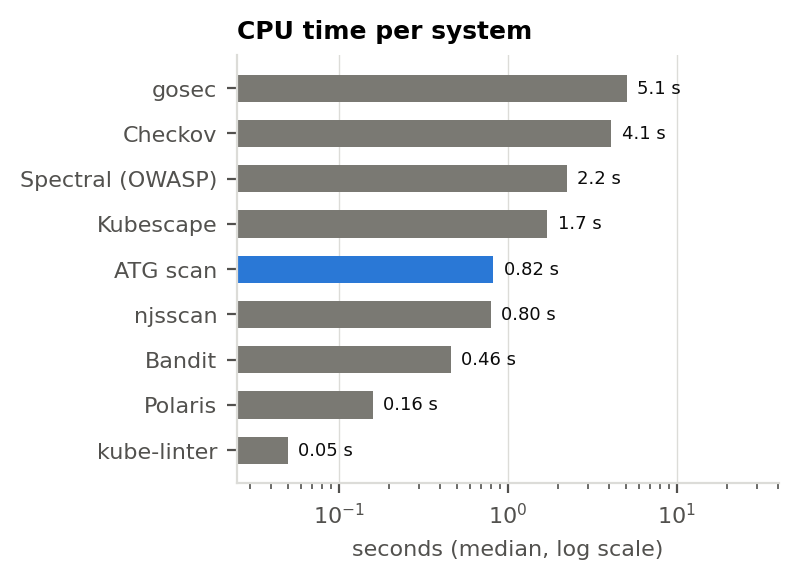
\includegraphics[width=\columnwidth]{figs/fig_cpu.png}
\caption{CPU time to review one system (median, log scale). ATG: the ATG and PostgreSQL containers during the scan.}
\label{fig:cpu}
\end{figure}

\begin{figure}[!htbp]
\centering
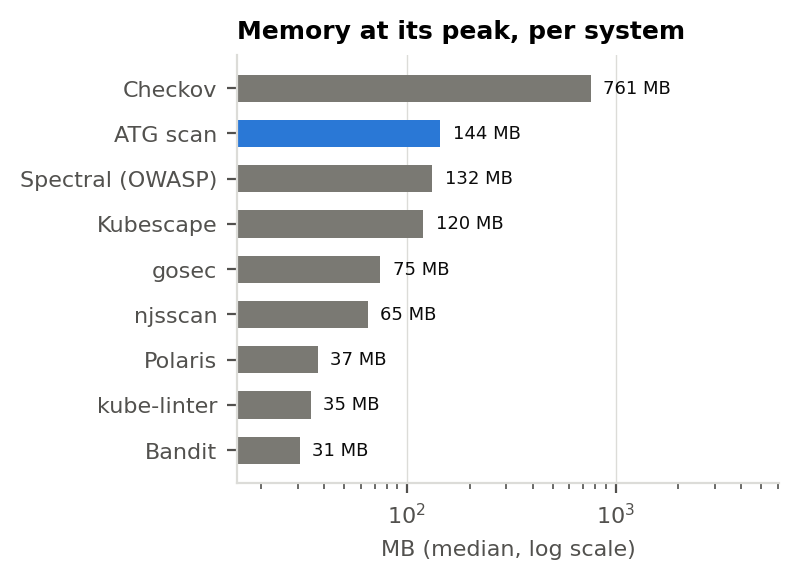
\includegraphics[width=\columnwidth]{figs/fig_memory.png}
\caption{Peak memory to review one system (median, log scale). ATG: the ATG and PostgreSQL containers during the scan.}
\label{fig:mem}
\end{figure}

\textit{ATG's whole review.} Unlike the file scanners, ATG is also running while the users send their requests. Table~\ref{tab:containers} splits its use over its four containers and over the two stages of a review. While the users run, the sidecar does most of the work: 1.5~s of CPU per system, or 2.4~ms of CPU for each request it carries (median; 2.0--2.7~ms). During the scan the ATG container uses 0.69~s and PostgreSQL 0.16~s. All four containers together used 2.8~s of CPU time over a whole review (5.1~s at most) and held at most 232~MB at once (260~MB on the largest system). They read and wrote nothing on disk, because ATG keeps the captured traffic and its database in memory, and the median container received and sent under 0.5~MB over the network in a review (the sidecar's traffic counts twice: in from a caller and out to the service, and back).

\begin{table*}[!t]
\caption{What ATG's four containers use during a review: median over the ten systems, in brackets the most. Users running: the system's users send their requests through the sidecar; scan: Phases 1--4}
\label{tab:containers}
\centering
\scriptsize
\setlength{\tabcolsep}{3pt}
\begin{tabular}{@{}l>{\raggedright\arraybackslash}p{3.6cm}rrrrrrr@{}}
\toprule
Container & Role & CPU, users running & CPU, scan & Peak memory & Average memory & Network in / out & Disk read / write & Processes \\
\midrule
%%containers%%
\bottomrule
\end{tabular}
\end{table*}

\FloatBarrier
\subsection{Accuracy}\label{sec:eval-acc}
This part asks how many of the 712 known weaknesses each tool finds, and how complete ATG's API inventory is. The known weaknesses fall into three groups. \textit{Configuration} (546) are mistakes in the deployment files (Kubernetes manifests, Docker Compose files, gateway settings), for example a container that may run as root, no network policy, no memory or CPU limit, a password written in a plain file, an image without a fixed version, or a public entry without HTTPS; the Kubernetes scanners and ATG can find these. \textit{API behaviour} (82) is how the running API behaves when it is used, for example an operation that returns private data without a login, one service calling another without credentials, an admin or debug page open to everyone, a password sent in the URL, or a login with no limit on wrong tries; only a tool that sees the API in use (ATG) or reads its API document (Spectral and Checkov's OpenAPI checks, partly) can find these. \textit{Inventory and visibility} (84) is what the owners do not know about their own APIs, for example operations that no API document describes (shadow APIs) and services that send no traces; only ATG compares what runs with what is documented.

\begin{figure}[!htbp]
\centering
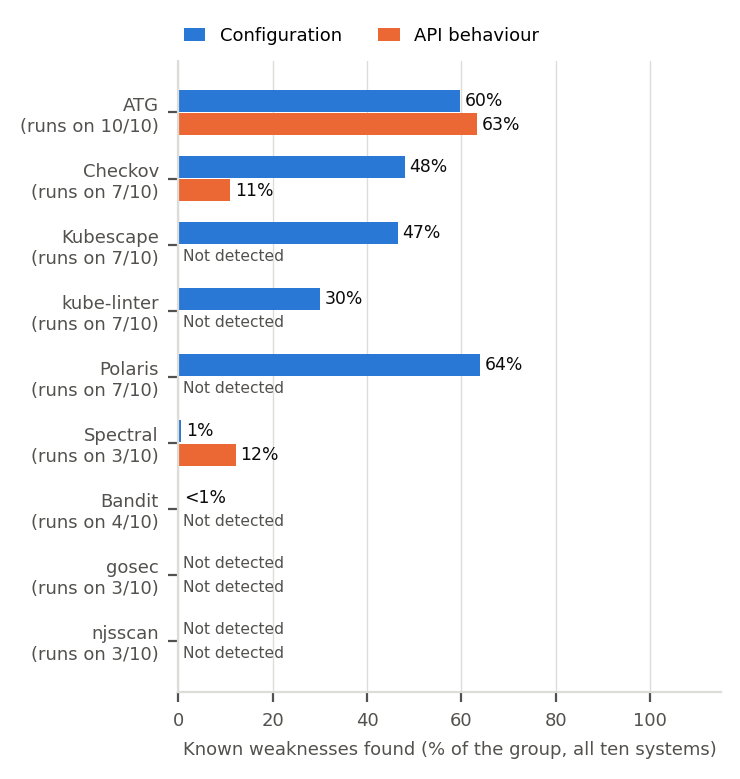
\includegraphics[width=\columnwidth]{figs/fig_oss_groups.png}
\caption{Known weaknesses found in the configuration and API-behaviour groups; in brackets, the number of systems each tool can run on. Inventory and visibility is in Table~\ref{tab:inventory}.}
\label{fig:tools}
\end{figure}

\textit{Inventory and visibility: detected or not.} Finding these needs the running system compared with the API documents and the deployment files, so it is a capability a tool either has or does not have. Table~\ref{tab:inventory} therefore shows it as detected or not detected rather than as a score, and Fig.~\ref{fig:tools} leaves it out. ATG detects all 58 operations and services without an API document and all 26 services that send no traces; none of the other tools detects either.

\begin{table}[!htbp]
\caption{Inventory and visibility: detected or not}
\label{tab:inventory}
\centering
\scriptsize
\setlength{\tabcolsep}{3pt}
\begin{tabular}{@{}l>{\raggedright\arraybackslash}p{2.3cm}>{\raggedright\arraybackslash}p{1.8cm}>{\raggedright\arraybackslash}p{2.0cm}@{}}
\toprule
Tool & Shadow APIs and services without an API document & Services that send no traces & Inventory and visibility (84) \\
\midrule
%%inventory%%
\bottomrule
\end{tabular}
\end{table}

\textit{Operations ATG listed.} No other tool lists a system's operations, so the inventory is measured for ATG alone (Table~\ref{tab:ops}). Of the 201 operations in the systems' code, ATG's inventory from the same \texttt{DEMO-ALL} run lists 189 (94\%), and 189 of its 212 entries (89\%) are real operations; an operation listed twice, for example once at the gateway and once at the service, counts as one wrong entry. All 23 wrong entries come from two systems. In Acme Air the Ingress controller is the gateway for five services, and ATG lists their operations a second time under the controller (15 entries). In FTGO the gateway's routes are written in Java code, which ATG does not read, so 8 of its entries stay under the gateway and are not matched to the services behind it. Runtime sources see only what is used, so an operation that the users never call and no document lists stays invisible.

\begin{table}[!htbp]
\caption{Operations ATG listed (its API inventory) against every operation in the systems' code. Correct: the share of ATG's entries that are real operations}
\label{tab:ops}
\centering
\footnotesize
\setlength{\tabcolsep}{3pt}
\begin{tabular}{@{}lrrrr@{}}
\toprule
System & In the code & Listed correctly & ATG's entries & Correct \\
\midrule
%%ops%%
\bottomrule
\end{tabular}
\end{table}

\textit{How many known weaknesses each tool found.} Table~\ref{tab:tools} counts, for each tool, the known weaknesses it found of all 712, so a tool that cannot read a system scores 0 there; the known weaknesses it found of what it can check, that is, of the kinds it has a check for on the systems it can read; and its correct reports, the share of its reports (kind and place) that are in the answer key. The rest are false alarms or problems the answer key does not list.

ATG finds 462 of the 712 (65\%), and 714 of its 950 reports (75\%) match a known weakness. The best other tool, Polaris, finds 349 (49\%) with 95\% of its reports correct, followed by Checkov (271), Kubescape (254) and kube-linter (164); Spectral finds 13 and the three code scanners 1 together. On configuration Polaris finds a little more than ATG (64\% against 60\%). The two check different things: ATG has no rule for container hardening (C9, 97 known weaknesses) or mounted service-account tokens (C10, 72), and it reports missing resource limits only on services the internet reaches, while Polaris cannot read the three Compose systems. On API behaviour ATG finds 52 of 82 (63\%). The most any other tool finds is 10 (Spectral) and 9 (Checkov's OpenAPI checks), both only on the three systems that have an API document.

\begin{table*}[!t]
\caption{How many known weaknesses each tool found (712 known weaknesses on the ten systems). Inventory and visibility is in Table~\ref{tab:inventory}}
\label{tab:tools}
\centering
\scriptsize
\setlength{\tabcolsep}{4pt}
\begin{tabular}{@{}lrrrrrr@{}}
\toprule
Tool & Systems it can read & Found (of 712) & Configuration & API behaviour & Found, of what it can check & Correct reports \\
\midrule
%%found%%
\bottomrule
\end{tabular}
\end{table*}

\textit{ATG's reports that are not in the answer key.} 236 of ATG's 950 reports (25\%) match no known weakness. 147 are inventory reports: 98 are on workloads the answer key does not count as API services (databases, caches, message brokers, registries, monitoring, load generators and web front ends), and 49 are on operations, mostly the extra entries in Acme Air and FTGO. 62 report a sensitive operation without authentication on operations that have no authentication check but that the answer key does not count as sensitive; most serve public data, such as a catalogue or a flight search. The remaining 27 are 9 bulk-sensitive-data reports, 8 debug-endpoint reports, 6 services published outside the gateway, 3 broken-object-level-authorization reports and 1 login without a rate limit.

\textit{Why the file scanners find configuration but no API behaviour or inventory.} API behaviour is how the running API answers: who may call an operation, what it returns, whether one service calls another without credentials. Kubernetes and Compose files do not describe API operations at all, and code scanners look for coding mistakes, not for who may call what. Only an API document says something about the API, which is why Spectral and Checkov's OpenAPI checks find a few API-behaviour weaknesses where a document exists; even there, the OWASP ruleset of Spectral, in its own description, ``cannot see what is happening in your code''. Inventory and visibility compare what runs with what is documented and traced, and a tool that reads one kind of file has nothing to compare it with.

Section~\ref{sec:discussion} checks that these zeros are not a scoring gap by listing every check the tools reported.

\textit{Found, by kind of weakness.} Table~\ref{tab:kinds} breaks the result down by kind. ATG finds every known case of containers that may run as root (90), mutable image tags (71), services published outside the gateway (16), missing network segmentation (109), credentials in a URL (3), bulk sensitive data (3), missing API documents (58) and missing traces (26). Its weakest kinds are exposed admin functions (1 of 7) and debug endpoints (2 of 7), whose paths (\texttt{/loader/load}, \texttt{/memory}) do not follow the names the rules know or which are whole consoles such as Spring Boot Admin, and missing resource limits (19 of 58). ATG reports missing resource limits (C3) only for services reachable from the internet, where they matter for API4 (resource consumption); the scanners report every container, which is why they find more C3 cases.

\begin{table*}[!t]
\caption{Found, by kind of weakness (the two kinds without known weaknesses in these systems, A8 SSRF-prone input and C2 privileged container, are left out). $\cdot$: the tool has no check for this kind}
\label{tab:kinds}
\centering
\scriptsize
\setlength{\tabcolsep}{3.5pt}
\begin{tabular}{@{}l>{\raggedright\arraybackslash}p{4.6cm}rrrrrrrrrr@{}}
\toprule
Code & Kind of weakness & Known & ATG & Checkov & Kubescape & kube-linter & Polaris & Spectral & Bandit & gosec & njsscan \\
\midrule
%%kinds%%
\bottomrule
\end{tabular}
\end{table*}

\textit{Found on each system.} Fig.~\ref{fig:persystem} and Table~\ref{tab:persystem} give the result per system, against each system's own answer key. ATG finds the most on four systems (Online Boutique and the three Compose systems), ties on Bookinfo, and finds fewer than the best Kubernetes scanner on the other five. On the seven Kubernetes systems Polaris finds 349 and ATG 304, mostly because of the container-hardening and service-account-token checks ATG does not have (125 of Polaris's finds). ATG's overall lead comes from the three Compose systems, where it finds 158 and no Kubernetes scanner can run, and from the API-behaviour and inventory kinds.

\begin{figure*}[!t]
\centering
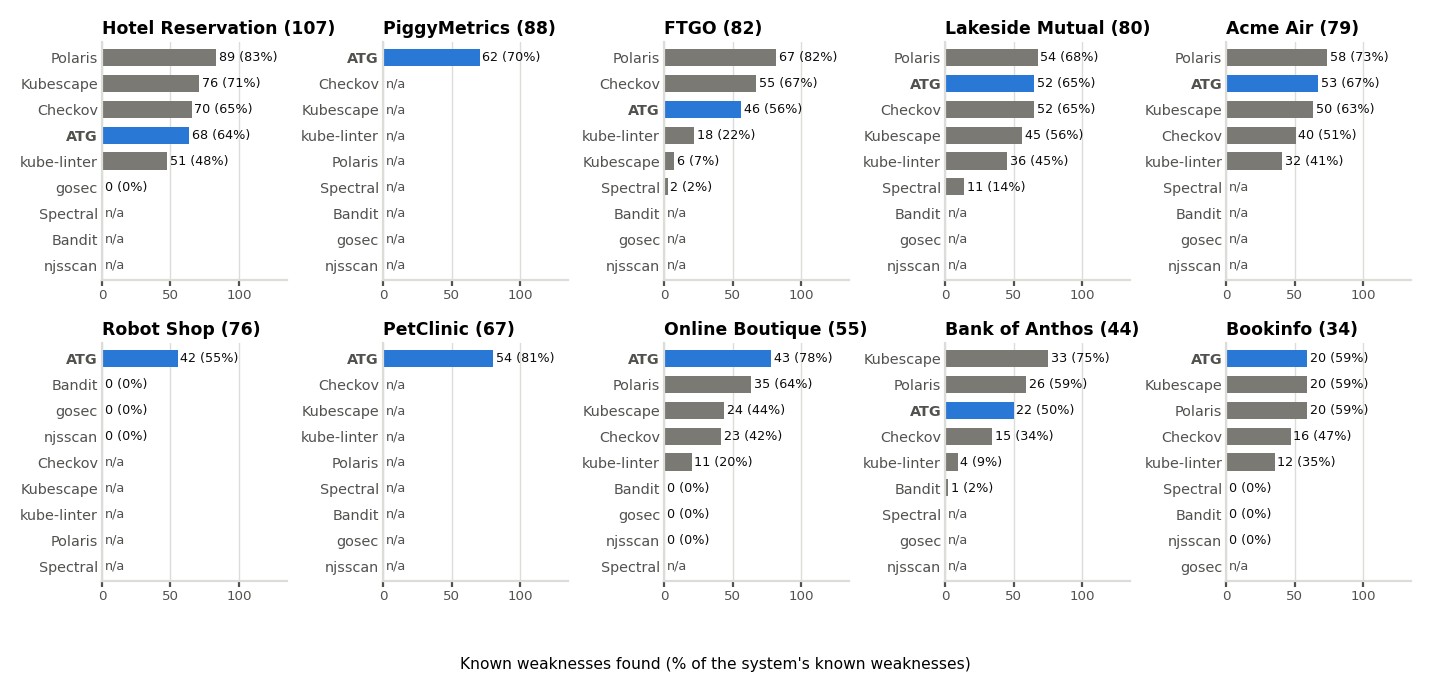
\includegraphics[width=\textwidth]{figs/fig_systems_grid.png}
\caption{Known weaknesses found on each system by every tool, the systems with the most known weaknesses first (in brackets, the system's known weaknesses). n/a: the tool cannot read that system's files.}
\label{fig:persystem}
\end{figure*}

\begin{table*}[!t]
\caption{Found on each system, the systems with the most known weaknesses first. n/a: the tool cannot read that system's files; 0: it ran and found none}
\label{tab:persystem}
\centering
\scriptsize
\setlength{\tabcolsep}{4pt}
\begin{tabular}{@{}lrrrrrrrrrr@{}}
\toprule
System & Known & \textbf{ATG} & Checkov & Kubescape & kube-linter & Polaris & Spectral & Bandit & gosec & njsscan \\
\midrule
%%persys%%
\bottomrule
\multicolumn{11}{@{}l}{\scriptsize $^{c}$Docker Compose.}
\end{tabular}
\end{table*}

\textit{ATG and a Kubernetes scanner used together.} Because ATG and the Kubernetes scanners check different things, their results add up. The scanners add the container-hardening checks ATG does not have (C9, C10), and ATG adds the API, inventory and Compose findings they cannot make. ATG finds 462 and Polaris 349; 202 are found by both, so the pair finds 609 of the 712 (86\%). With Kubescape (254) the overlap is 130 and the pair finds 586 (82\%); with Checkov (271) the overlap is 122 and the pair finds 611 (86\%). Measured on the same answer key, every combination gives: ATG alone 462 (65\%), ATG and Polaris 609 (86\%), ATG and Checkov 611 (86\%), ATG, Polaris and Kubescape 616 (87\%), ATG and the four Kubernetes scanners 619 (87\%), and ATG and all eight tools 622 (87\%). ATG with the three code scanners (Bandit, gosec, njsscan) still finds 462 (65\%), so they add nothing, and the eight tools without ATG find 370 (52\%).

Even all nine tools together leave 90 of the 712 known weaknesses unfound. Section~\ref{sec:conclusion} lists what ATG and every tool still miss, by kind, and turns it into the future plan.

\FloatBarrier
\subsection{Systems covered}\label{sec:eval-sys}
This part asks on how many of the ten systems each tool can run at all (Fig.~\ref{fig:reach}). ATG runs on all ten: it needs a running test deployment, in any language, and reads whatever files the system has. The four Kubernetes scanners need Kubernetes manifests (Kubescape also needs current API versions) and cannot read Docker Compose, so all four skip Robot Shop, PetClinic and PiggyMetrics; Checkov has no Docker Compose checks, and the other three read Kubernetes manifests only. Kubescape also ran on FTGO but found only 6 of its 82 known weaknesses, because FTGO declares its Deployments and StatefulSets with API versions Kubernetes has removed (\texttt{extensions/v1beta1}, \texttt{apps/v1beta1}) and Kubescape skipped them, scanning only the Services, the Secret and the Job; the other scanners read them. Spectral needs an OpenAPI document, which only Lakeside Mutual, FTGO and Bookinfo have, so it could not read the other seven: Online Boutique, Bank of Anthos, Robot Shop, Acme Air, PetClinic, PiggyMetrics and Hotel Reservation. Each code scanner needs a service in its language. Bandit found Python in four systems and could not read the six without a Python service (Acme Air, PetClinic, PiggyMetrics, Lakeside Mutual, FTGO and Hotel Reservation). gosec found Go in three and could not read the seven without a Go service (Bank of Anthos, Acme Air, PetClinic, PiggyMetrics, Lakeside Mutual, FTGO and Bookinfo). njsscan found Node.js in three and could not read the seven without a Node.js service (Bank of Anthos, Acme Air, PetClinic, PiggyMetrics, Lakeside Mutual, FTGO and Hotel Reservation).

\begin{figure}[!htbp]
\centering
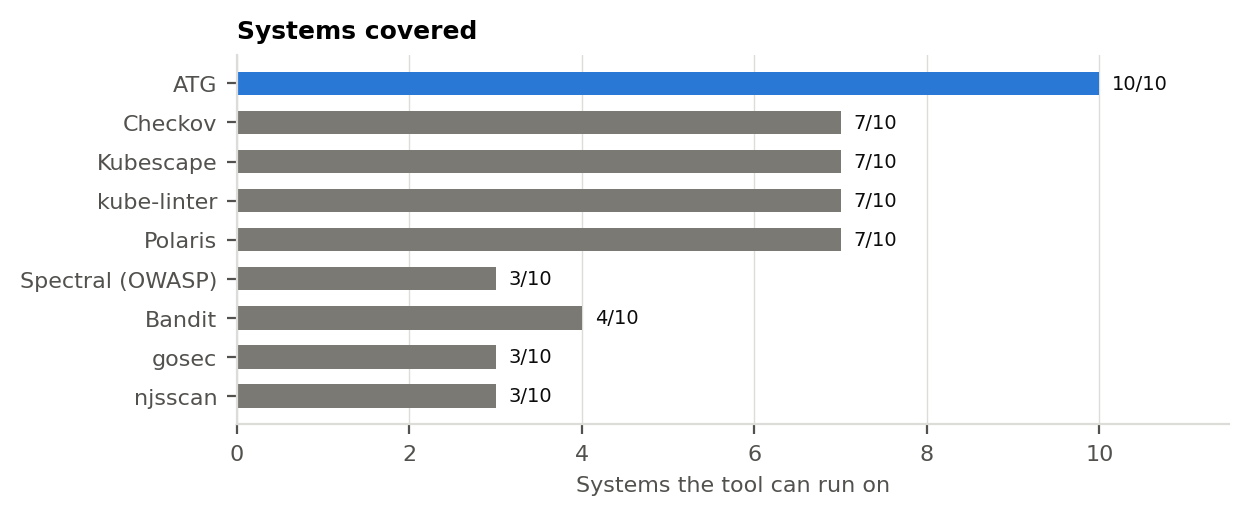
\includegraphics[width=\columnwidth]{figs/fig_systems_covered.png}
\caption{Systems each tool can run on, of the ten.}
\label{fig:reach}
\end{figure}

\FloatBarrier
\subsection{Language limits}\label{sec:eval-lang}
This part asks which services, and which programming languages, each tool can review. The 65 services of the ten systems are written in eight languages: Java (35 services), Go (13), Python (7), Node.js (6), and C\#, Ruby, PHP and JavaScript served to the browser (one each). Figs.~\ref{fig:services} and~\ref{fig:langs} and Table~\ref{tab:langs} count, for each tool, the services it could review and their languages; Table~\ref{tab:syslangs} lists every service of each system with its language.

The three code scanners read one language each. Bandit could read 7 services, gosec 13 and njsscan 6, so together they read 26 of the 65 (40\%), and no free scanner in this comparison reads the 35 Java services or the C\#, Ruby, PHP and browser JavaScript ones. Five of the ten systems (Acme Air, PetClinic, PiggyMetrics, Lakeside Mutual and FTGO) are written only in Java, so none of their services was read by a code scanner. The Kubernetes scanners and Spectral do not read code, so their limit is the kind of file rather than the language: the Kubernetes scanners reach the 44 services deployed with Kubernetes files, in six languages, and Spectral the 7 services that an API document describes, in Java and Python. ATG does not read code either. It reviews the running services through their HTTP traffic and traces, and it reads all their files, so it reviewed all 65 services in all eight languages. By language, the Java services (35) were reviewed by ATG, the four Kubernetes scanners and Spectral, but by no code scanner; Go (13) by ATG, the Kubernetes scanners and gosec; Python (7) by ATG, the Kubernetes scanners, Spectral and Bandit; Node.js (6) by ATG, the Kubernetes scanners and njsscan; C\# and Ruby (one service each) by ATG and the Kubernetes scanners; and PHP and the browser JavaScript, both in Robot Shop, a Compose system, only by ATG.

\begin{figure}[!htbp]
\centering
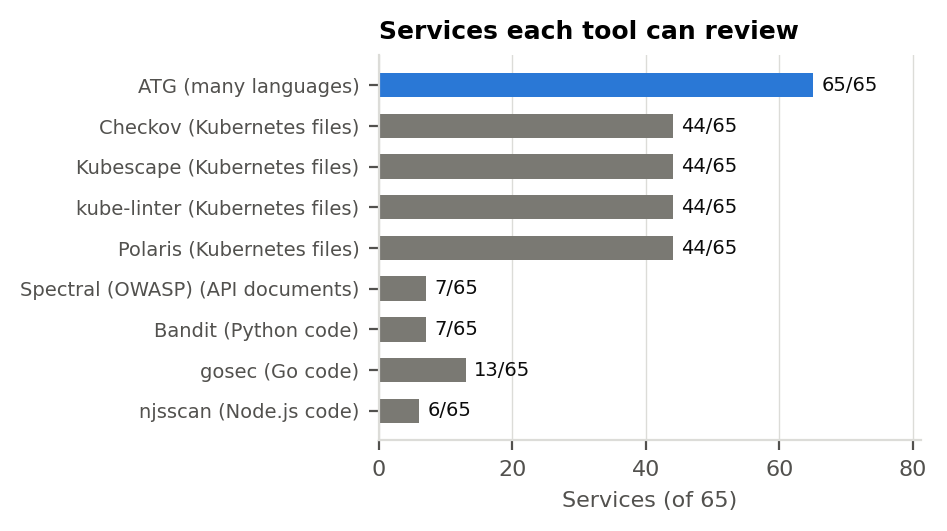
\includegraphics[width=\columnwidth]{figs/fig_services.png}
\caption{Services each tool can review, of the 65.}
\label{fig:services}
\end{figure}

\begin{figure}[!htbp]
\centering
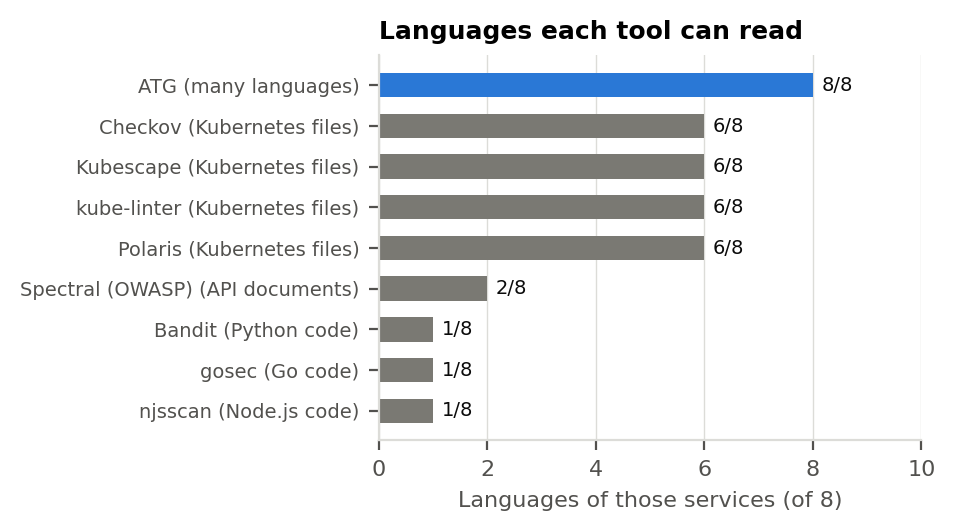
\includegraphics[width=\columnwidth]{figs/fig_languages.png}
\caption{Languages of the services each tool can review, of the eight.}
\label{fig:langs}
\end{figure}

\begin{table}[!htbp]
\caption{Services and languages each tool can review (of 65 services and eight languages)}
\label{tab:langs}
\centering
\scriptsize
\setlength{\tabcolsep}{2.5pt}
\begin{tabular}{@{}>{\raggedright\arraybackslash}p{1.35cm}>{\raggedright\arraybackslash}p{1.5cm}rr>{\raggedright\arraybackslash}p{2.75cm}@{}}
\toprule
Tool & What it reads & Services & Lang. & Which languages \\
\midrule
%%langs%%
\bottomrule
\end{tabular}
\end{table}

\begin{table*}[!t]
\caption{The services of each system and their languages, and the services each code scanner can read (Bandit: Python, gosec: Go, njsscan: Node.js)}
\label{tab:syslangs}
\centering
\scriptsize
\setlength{\tabcolsep}{3pt}
\begin{tabular}{@{}lr>{\raggedright\arraybackslash}p{2.5cm}>{\raggedright\arraybackslash}p{8.4cm}rrr@{}}
\toprule
System & Services & Languages & Each service (language) & Bandit & gosec & njsscan \\
\midrule
%%syslangs%%
\bottomrule
\end{tabular}
\end{table*}

